In the seminal paper by Einstein \cite{einstein_uber_1905}, that laid foundations to Quantum Mechanics, Einstein postulated that light is made of discrete quanta of energy $E = h\nu$ to explain the observations by Hertz and J.J. Thompson; explaining the photoelectric effect. The effect can be described by the Equation \ref{eq:photoelectric} where $E_e$ the emitted kinetic energy, $h$ is the plank's constant, $\nu$ the frequency of the incoming photon and  $\phi$ the material-specific work function (also known as binding energy).

\begin{equation}\label{eq:photoelectric}
    E_e = h\nu - \phi
\end{equation}

The equation describes how incident photons on a surface eject photoelectrons, provided the photon energy $h\nu$ exceeds $\phi$. This also highlights that the emitted kinetic energy $E_e$ does not depend on the photon flux (photon counts per second). However, the flux increases the total amount of electrons released from the material.

It is then apparent that the binding energy of electrons can be found by irradiating light onto the material and measuring the $E_e$ of photoelectrons. \gls{PES}, is exactly such a technique that leverages this principle to probe the electronic structure of materials.

\section{Where PES is performed}
Table top, Synchrotrons, FELs. Time resolved PES and how it relates to acquisition times.

\begin{figure}
    \centering
    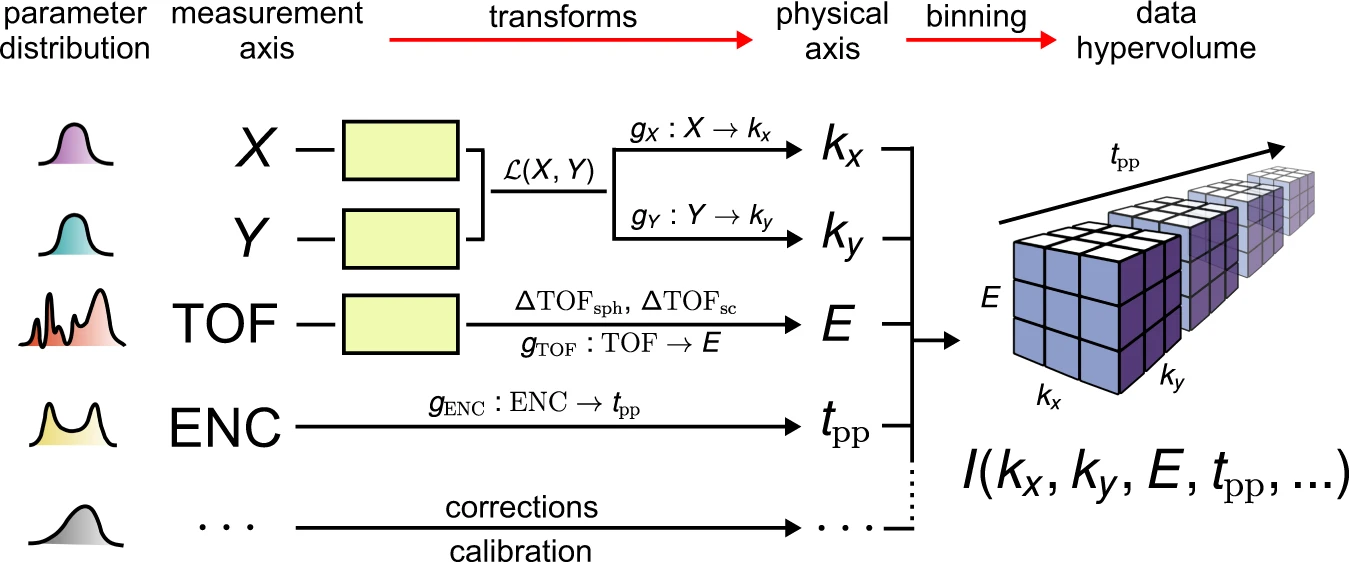
\includegraphics[width=1\linewidth]{images/2024-08-25-22-36-44.png}
    \caption{MPES taken from \cite{xian_open-source_2020}}
    % \label{fig:enter-label}
\end{figure}



\section{HEXTOF Setup at FLASH}
\gls*{DESY} is a national 
\begin{figure}
    \centering
    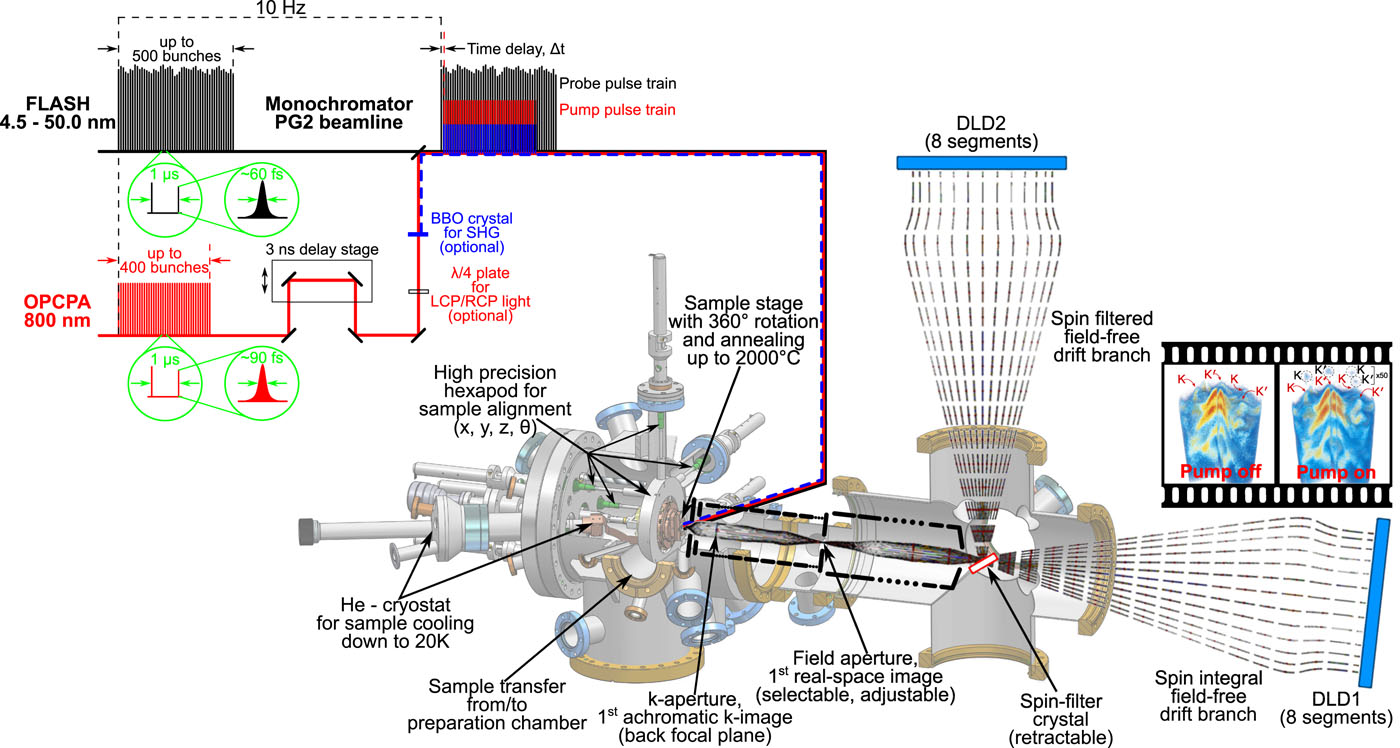
\includegraphics[width=1\linewidth]{images/2024-08-27-10-50-01.png}
    \caption{HEXTOF taken from \cite{kutnyakhov_time-_2020}}
    % \label{fig:enter-label}
\end{figure}



\section{Describing the data GdW, WSe2, GrIr, and new one}

\section{Creating the dataset Corrections Calibrations etc}

\section{Using CLT}
% Central Limit Theorem (CLT)
The \textbf{Central Limit Theorem} states that for a sequence of i.i.d. random variables \(X_1, X_2, \ldots, X_n\) with mean \( \mu \) and variance \( \sigma^2 \), the normalized sum of these variables approaches a standard normal distribution as \(n\) tends to infinity:

\[
\frac{\sum_{i=1}^{n} X_i - n\mu}{\sigma \sqrt{n}} \xrightarrow{d} N(0, 1) \quad \text{as} \quad n \to \infty.
\]

This convergence is in distribution.
